\documentclass{article}
\usepackage{amsmath}
\usepackage{booktabs}
\usepackage{pgfplots}
\usepackage{float}
\pgfplotsset{compat=1.18}

\newcommand\plotmulti{.8}

\title{CS 4033/5033 Project 3}
\author{Alexander Gréus, Spencer Smith}
\date{}

\begin{document}
\maketitle

\section{Clustering methods}
% List the clustering method you chose for this project and explain why you chose this clustering method

We chose K-Means clustering because it is simple and works well for grouping similar data. It splits the data into a set number of clusters based on how close points are to a center. It is also quick to run and easy to understand, which made it a good fit for our project.

\section{Goodness measure}
% List and justify the “goodness” measure(s) you will use to evaluate the quality of clustering accomplished for each dataset.

As goodness measure we chose Silhouette Score which ranges from -1 to 1. Higher values mean better-defined clusters. We tested this score for $k$ clusters between 2 and 8 and chose the $k$ with the best score.

\section{Graphical representation}
% List and justify any graphical representation(s) you will use to understand the data itself and the clustering performance.

We plotted the data using 2d and 3d scatter plots while the color of the points represent the selected cluster. Additionally, we plotted the Silhouette Score of each dataset for $k$ and for $k-1$ and $k+1$.

% Implement clustering code for your project. Alternately, you may use existing clustering software or services. If you choose this alternative, describe and justify your choice of software/services. Note that only software/services readily available to all OU students (including your TA) may be selected.

% For each dataset, conduct clustering and collect performance data.

% Report your results, analysis, and conclusions regarding the application of clustering to each dataset individually and in combination. Be sure to consider how performance varies as complexity of the data varies.

% For each dataset, include the number of clusters found, the points for each cluster found (in a separate csv file for each cluster), and any graphics you selected to support your analysis.

% If your chosen clustering method categorizes some points as “noise” (or otherwise excludes them from the clusters found), include those points in their own csv file for each dataset.

% If your chosen clustering method requires you to choose the number of clusters k, explain how you chose k for each dataset and provide results for k − 1 and k + 1 in addition to your results for k.

\section{Clustering}

\subsection{Dataset 1}

Dataset 1 is best represented with 2 clusters. Figure \ref{fig:d1_silhouette} shows that the silhouette score for $k=2$ is highest and everything greater than $k=3$ has a bad score. The different clusters for $k=2$ can be seen in Figure \ref{fig:d1_clusterk} and for $k+1=3$ in Figure \ref{fig:d1_clusterk+1}.

\begin{figure}[h]
    \centering
    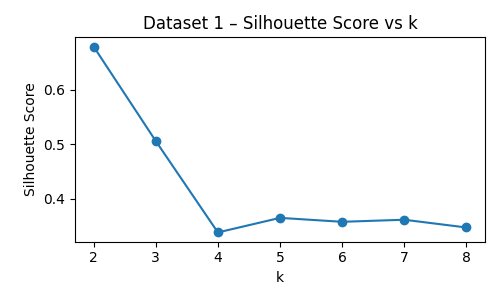
\includegraphics[width=\plotmulti\linewidth]{plots/Dataset1_Silhouette.png}
    \caption{Dataset 1 Silhouette Score vs $k$}
    \label{fig:d1_silhouette}
\end{figure}

\begin{figure}[h]
    \centering
    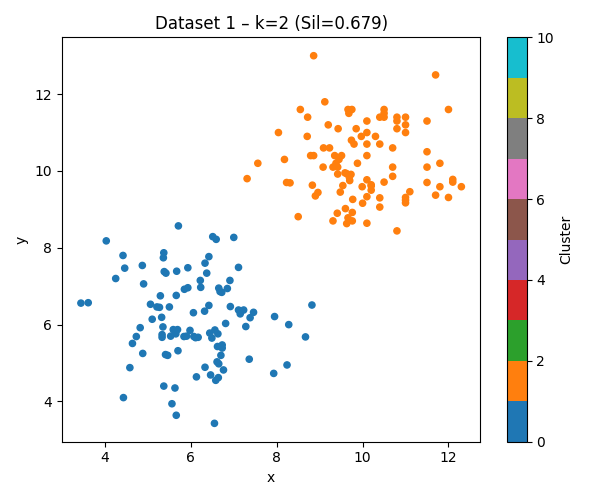
\includegraphics[width=\plotmulti\linewidth]{plots/Dataset1_k2.png}
    \caption{Dataset 1 Clustering with $k$ Clusters}
    \label{fig:d1_clusterk}
\end{figure}

\begin{figure}[h]
    \centering
    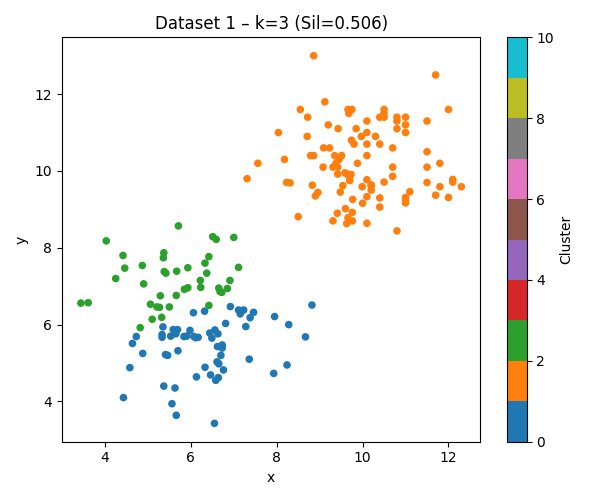
\includegraphics[width=\plotmulti\linewidth]{plots/Dataset1_k3.png}
    \caption{Dataset 1 Clustering with $k+1$ Clusters}
    \label{fig:d1_clusterk+1}
\end{figure}

\subsection{Dataset 2}

Dataset 2 is best represented with 2 clusters. Figure \ref{fig:d2_silhouette} shows that the silhouette score for $k=2$ is highest and everything greater than $k=3$ has a bad score. The different clusters for $k=2$ can be seen in Figure \ref{fig:d2_clusterk} and for $k+1=3$ in Figure \ref{fig:d2_clusterk+1}.

\begin{figure}[h]
    \centering
    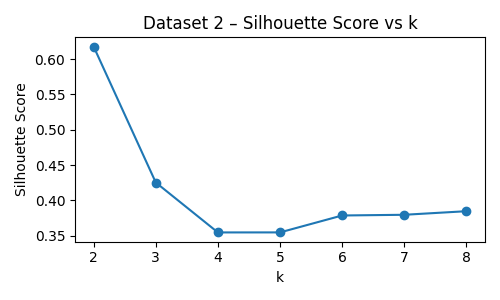
\includegraphics[width=\plotmulti\linewidth]{plots/Dataset2_Silhouette.png}
    \caption{Dataset 2 Silhouette Score vs $k$}
    \label{fig:d2_silhouette}
\end{figure}

\begin{figure}[h]
    \centering
    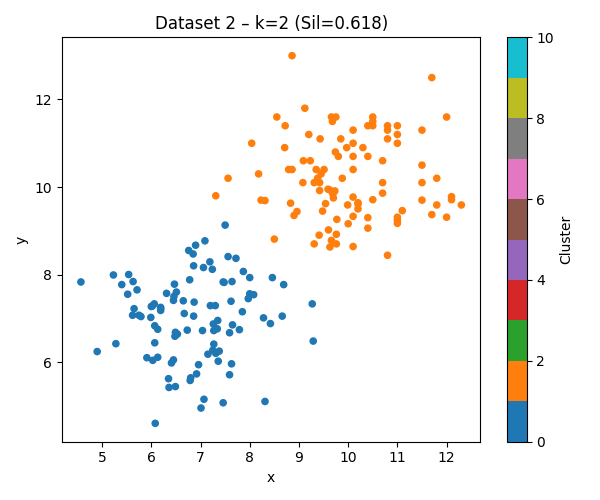
\includegraphics[width=\plotmulti\linewidth]{plots/Dataset2_k2.png}
    \caption{Dataset 2 Clustering with $k$ Clusters}
    \label{fig:d2_clusterk}
\end{figure}

\begin{figure}[h]
    \centering
    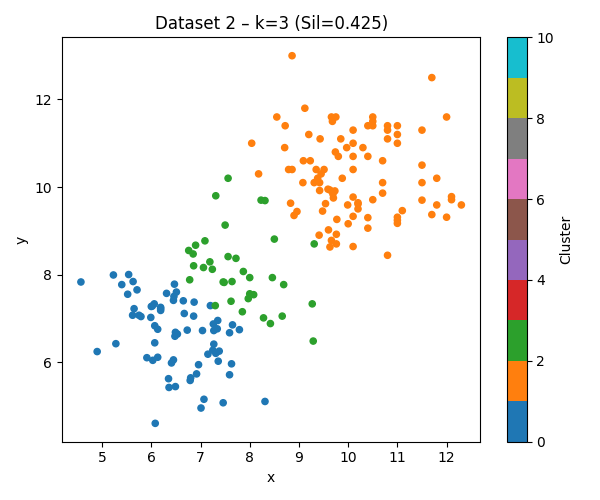
\includegraphics[width=\plotmulti\linewidth]{plots/Dataset2_k3.png}
    \caption{Dataset 2 Clustering with $k+1$ Clusters}
    \label{fig:d2_clusterk+1}
\end{figure}

\subsection{Dataset 3}

Dataset 3 is best represented with 8 clusters. Figure \ref{fig:d3_silhouette} shows that the silhouette score for $k=2$ is relatively high but the optimal is reached with higher $k$ values. The difference in the sillhouette score between $k$ values of 6, 7 or 8 is minimal. The different clusters for $k-1=7$ can be seen in Figure \ref{fig:d3_clusterk-1}, for $k=8$ in Figure \ref{fig:d3_clusterk} and for $k+1=9$ in Figure \ref{fig:d3_clusterk+1}.

\begin{figure}[h]
    \centering
    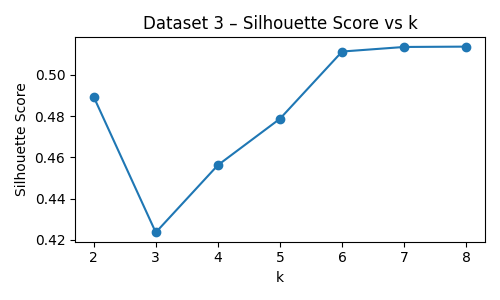
\includegraphics[width=\plotmulti\linewidth]{plots/Dataset3_Silhouette.png}
    \caption{Dataset 3 Silhouette Score vs $k$}
    \label{fig:d3_silhouette}
\end{figure}

\begin{figure}[h]
    \centering
    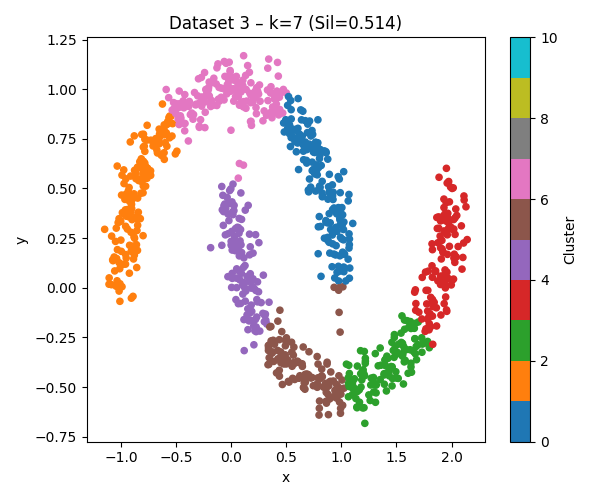
\includegraphics[width=\plotmulti\linewidth]{plots/Dataset3_k7.png}
    \caption{Dataset 3 Clustering with $k-1$ Clusters}
    \label{fig:d3_clusterk-1}
\end{figure}

\begin{figure}[h]
    \centering
    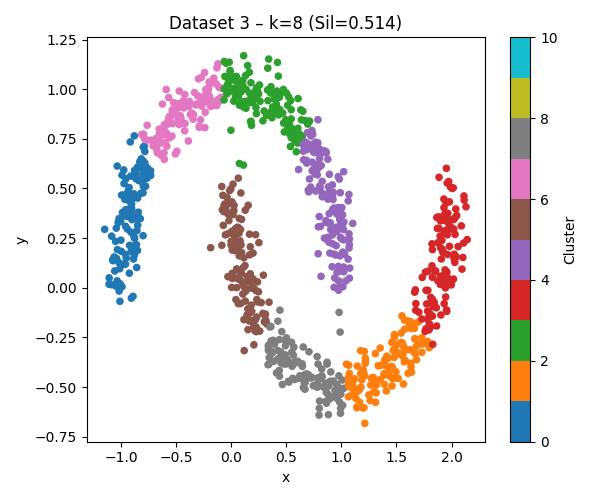
\includegraphics[width=\plotmulti\linewidth]{plots/Dataset3_k8.png}
    \caption{Dataset 3 Clustering with $k$ Clusters}
    \label{fig:d3_clusterk}
\end{figure}

\begin{figure}[h]
    \centering
    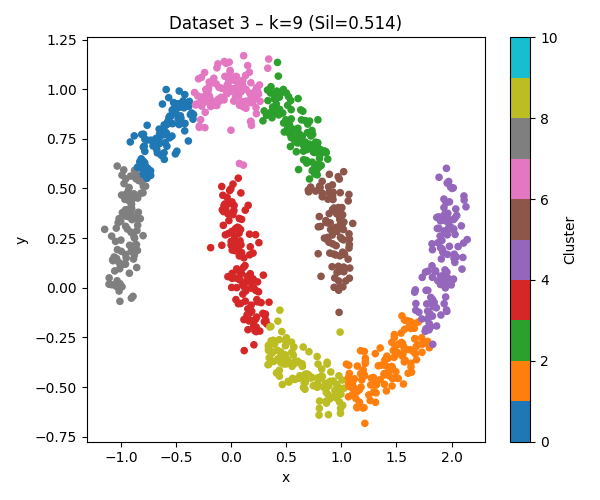
\includegraphics[width=\plotmulti\linewidth]{plots/Dataset3_k9.png}
    \caption{Dataset 3 Clustering with $k+1$ Clusters}
    \label{fig:d3_clusterk+1}
\end{figure}

\subsection{Dataset 4}

Dataset 4 is best represented with 7 clusters. Figure \ref{fig:d4_silhouette} shows that, similar to Dataset 3, the silhouette score for $k=2$ is relatively high but the optimal is reached with higher $k$ values. However, compared to Dataset 3 the difference between $k=2$ and higher $k$ values is only slight. Additionally, the difference in the sillhouette score between $k$ values of 6, 7 or 8 is minimal. The different clusters for $k-1=6$ can be seen in Figure \ref{fig:d4_clusterk-1}, for $k=7$ in Figure \ref{fig:d4_clusterk} and for $k+1=8$ in Figure \ref{fig:d4_clusterk+1}.

\begin{figure}[h]
    \centering
    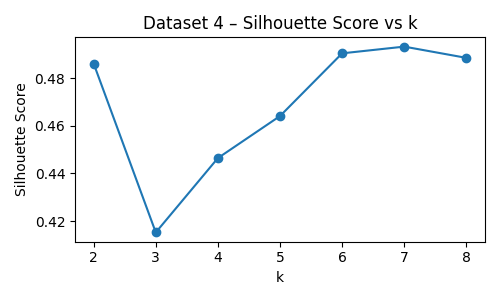
\includegraphics[width=\plotmulti\linewidth]{plots/Dataset4_Silhouette.png}
    \caption{Dataset 4 Silhouette Score vs $k$}
    \label{fig:d4_silhouette}
\end{figure}

\begin{figure}[h]
    \centering
    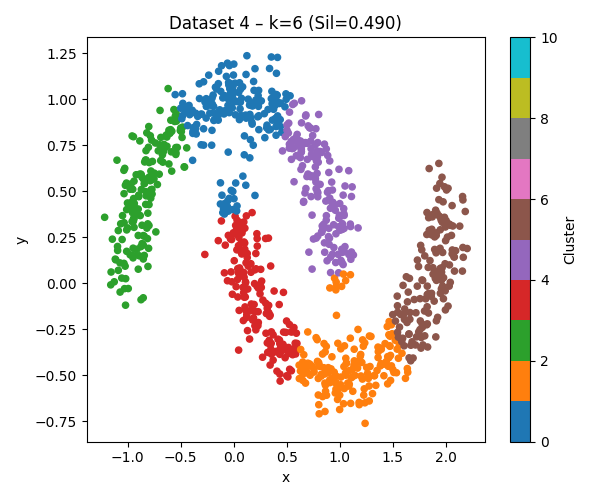
\includegraphics[width=\plotmulti\linewidth]{plots/Dataset4_k6.png}
    \caption{Dataset 4 Clustering with $k-1$ Clusters}
    \label{fig:d4_clusterk-1}
\end{figure}

\begin{figure}[h]
    \centering
    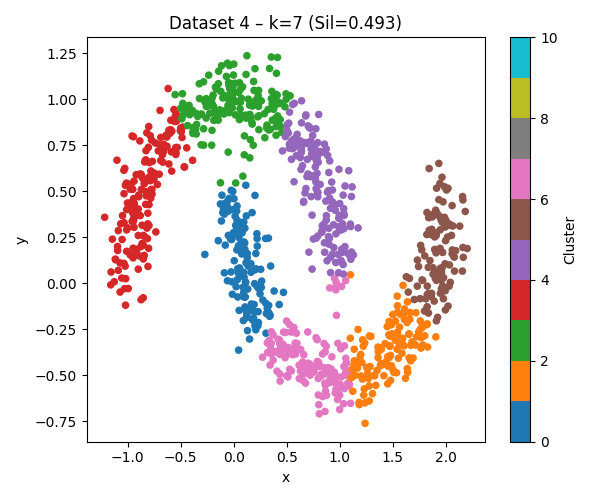
\includegraphics[width=\plotmulti\linewidth]{plots/Dataset4_k7.png}
    \caption{Dataset 4 Clustering with $k$ Clusters}
    \label{fig:d4_clusterk}
\end{figure}

\begin{figure}[h]
    \centering
    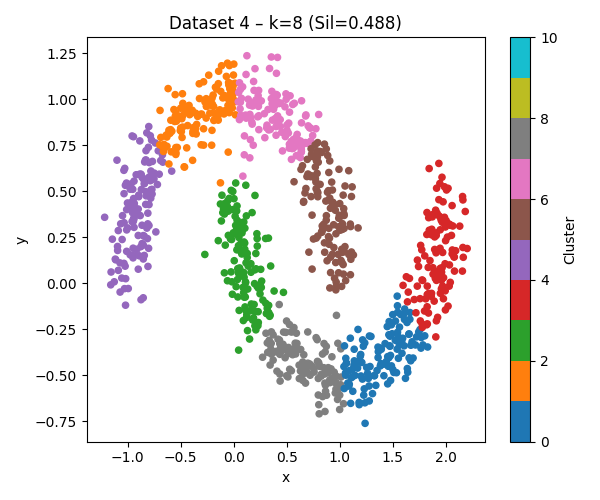
\includegraphics[width=\plotmulti\linewidth]{plots/Dataset4_k8.png}
    \caption{Dataset 4 Clustering with $k+1$ Clusters}
    \label{fig:d4_clusterk+1}
\end{figure}

\subsection{Dataset 5}

Dataset 5 is best represented with 4 clusters. Figure \ref{fig:d5_silhouette} shows that the silhouette scores for $k$ between 2 and 6 are relatively high but the optimal is reached at $k=4$. The different clusters for $k-1=3$ can be seen in Figure \ref{fig:d5_clusterk-1}, for $k=4$ in Figure \ref{fig:d5_clusterk} and for $k+1=5$ in Figure \ref{fig:d5_clusterk+1}.

\begin{figure}[h]
    \centering
    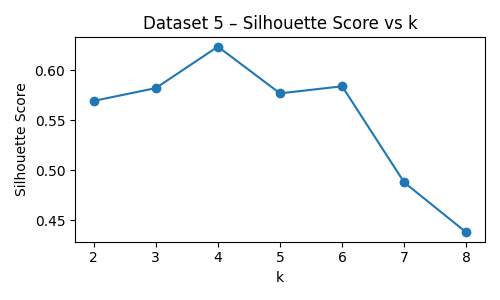
\includegraphics[width=\plotmulti\linewidth]{plots/Dataset5_Silhouette.png}
    \caption{Dataset 5 Silhouette Score vs $k$}
    \label{fig:d5_silhouette}
\end{figure}

\begin{figure}[h]
    \centering
    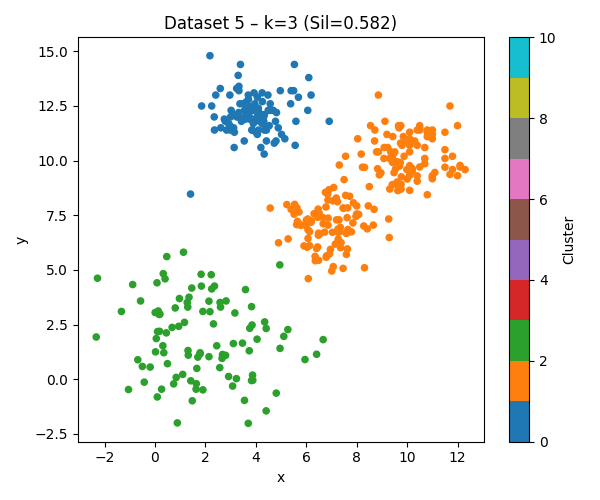
\includegraphics[width=\plotmulti\linewidth]{plots/Dataset5_k3.png}
    \caption{Dataset 5 Clustering with $k-1$ Clusters}
    \label{fig:d5_clusterk-1}
\end{figure}

\begin{figure}[h]
    \centering
    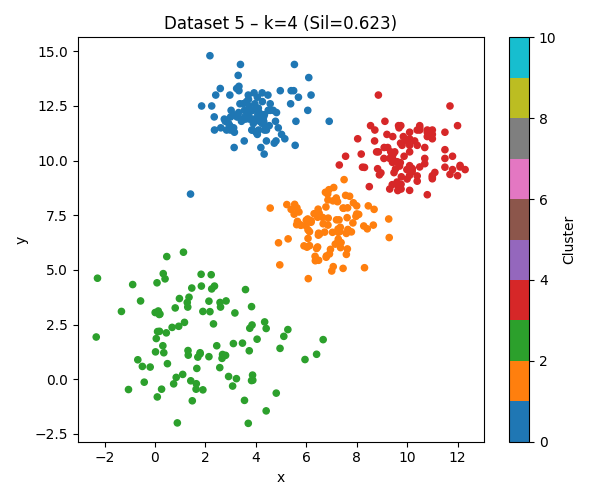
\includegraphics[width=\plotmulti\linewidth]{plots/Dataset5_k4.png}
    \caption{Dataset 5 Clustering with $k$ Clusters}
    \label{fig:d5_clusterk}
\end{figure}

\begin{figure}[h]
    \centering
    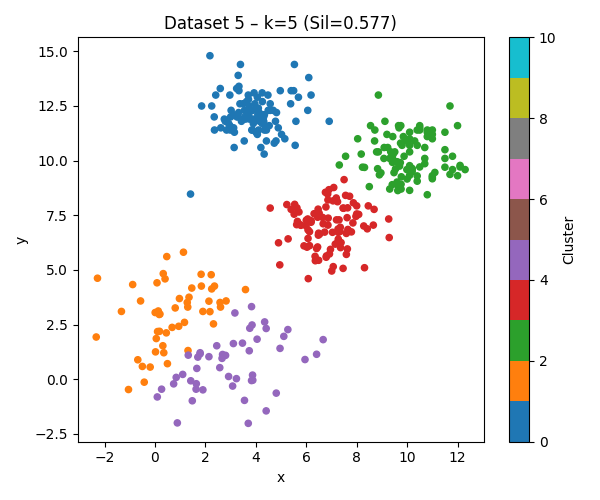
\includegraphics[width=\plotmulti\linewidth]{plots/Dataset5_k5.png}
    \caption{Dataset 5 Clustering with $k+1$ Clusters}
    \label{fig:d5_clusterk+1}
\end{figure}

\subsection{Dataset 6}

Dataset 6 is best represented with 2 clusters. Figure \ref{fig:d6_silhouette} shows that the silhouette score for $k=2$ is highest and everything greater than $k=3$ has a bad score. The different clusters for $k=2$ can be seen in Figure \ref{fig:d6_clusterk} and for $k+1=3$ in Figure \ref{fig:d6_clusterk+1}.

\begin{figure}[h]
    \centering
    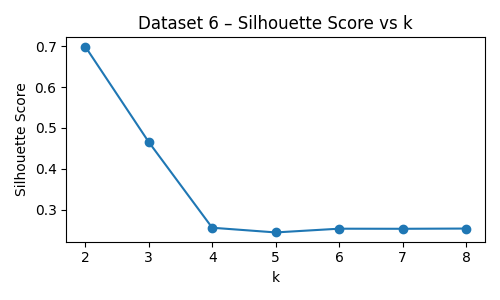
\includegraphics[width=\plotmulti\linewidth]{plots/Dataset6_Silhouette.png}
    \caption{Dataset 6 Silhouette Score vs $k$}
    \label{fig:d6_silhouette}
\end{figure}

\begin{figure}[h]
    \centering
    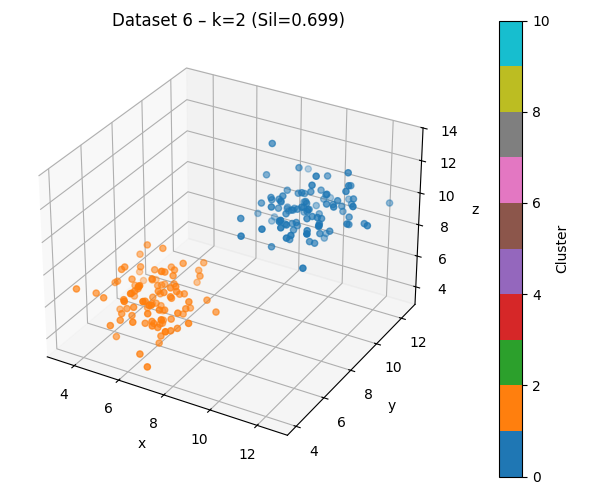
\includegraphics[width=\plotmulti\linewidth]{plots/Dataset6_k2.png}
    \caption{Dataset 6 Clustering with $k$ Clusters}
    \label{fig:d6_clusterk}
\end{figure}

\begin{figure}[h]
    \centering
    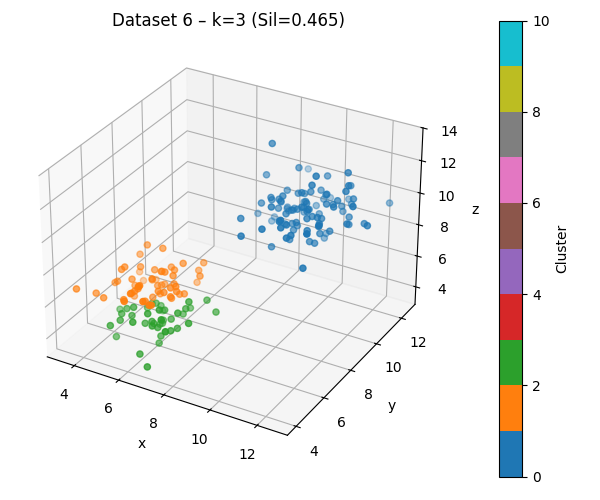
\includegraphics[width=\plotmulti\linewidth]{plots/Dataset6_k3.png}
    \caption{Dataset 6 Clustering with $k+1$ Clusters}
    \label{fig:d6_clusterk+1}
\end{figure}

\subsection{Dataset 7}

Dataset 7 is best represented with 2 clusters. Figure \ref{fig:d7_silhouette} shows that the silhouette score for $k=2$ is highest and everything greater than $k=3$ has a bad score. The different clusters for $k=2$ can be seen in Figure \ref{fig:d7_clusterk} and for $k+1=3$ in Figure \ref{fig:d7_clusterk+1}.

\begin{figure}[h]
    \centering
    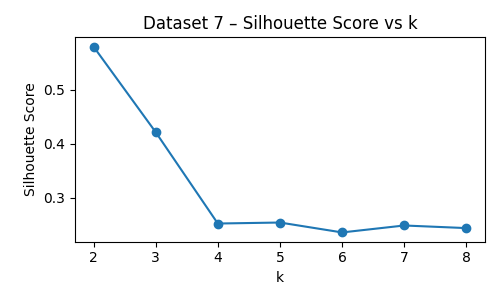
\includegraphics[width=\plotmulti\linewidth]{plots/Dataset7_Silhouette.png}
    \caption{Dataset 7 Silhouette Score vs $k$}
    \label{fig:d7_silhouette}
\end{figure}

\begin{figure}[h]
    \centering
    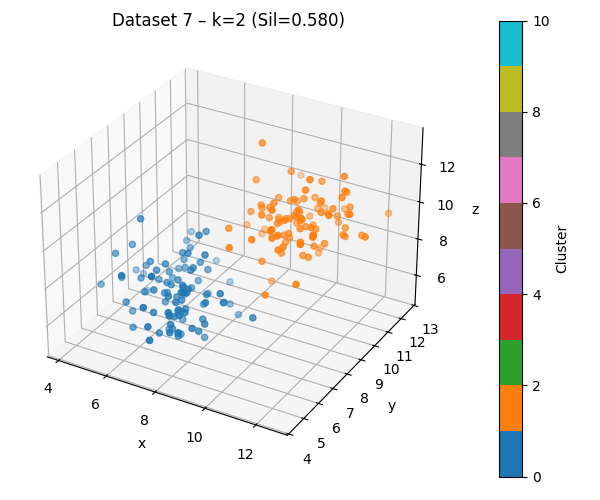
\includegraphics[width=\plotmulti\linewidth]{plots/Dataset7_k2.png}
    \caption{Dataset 7 Clustering with $k$ Clusters}
    \label{fig:d7_clusterk}
\end{figure}

\begin{figure}[h]
    \centering
    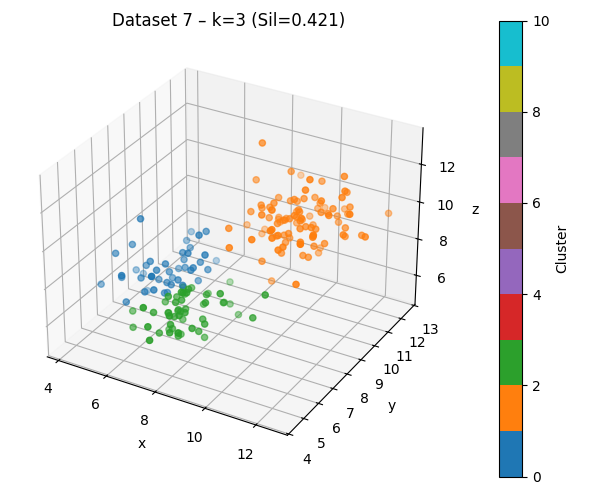
\includegraphics[width=\plotmulti\linewidth]{plots/Dataset7_k3.png}
    \caption{Dataset 7 Clustering with $k+1$ Clusters}
    \label{fig:d7_clusterk+1}
\end{figure}





\end{document}